\documentclass{beamer}
% \usetheme{Madrid}
\usepackage{tikz}
\usetikzlibrary{positioning}

\begin{document}
\title[CNN and GA To Play Draughts] % (optional, only for long titles)
{Improving CNN Draughts Evaluators using Genetic Algorithms}
\author[T. Nguyen] % (optional, for multiple authors)
{Thien Nguyen}
\institute[Durham] % (optional)
{
Department of Computer Science\\
Durham University
}
\subject{Computer Science}

% Title Frame
\frame{\titlepage}

\begin{frame}
  \frametitle{Outline}
  %Content goes here
    %An outline: What are the elements of your talk?
    \begin{block}{This is a Block}
        This is important information
     \end{block}
  
     \begin{alertblock}{This is an Alert block}
     This is an important alert
     \end{alertblock}
  
     \begin{exampleblock}{This is an Example block}
     This is an example 
     \end{exampleblock}
\end{frame}

% A title slide: Project title, student name, course, date
%  An outline: What are the elements of your talk?
% A problem description, possibly both informal and formal
% Motivation: Why do you want to solve this problem? Previous work, and how it relates to what you are doing
% Your approach to solving the problem
% What you have accomplished so far (not relevant for marking!) Analysis: How will you judge the outcome of your work?
% A conclusion slide: What did or will you accomplish?
% What still needs to be done
\begin{frame}
  \frametitle{Problem Description}
  \framesubtitle{A bit more information about this}
    % More content goes here
    % Why is it important?
    % Currently (except for AlphaGo Zero) are really good at exploiting human games and definining "intuition" from there.
\end{frame}

\begin{frame}
    \frametitle{Motivation}
    \framesubtitle{A bit more information about this}
    % Why do you want to solve this problem? Previous work, and how it relates to what you are doing
    %More content goes here
\end{frame}

% Neural Network Frame
\begin{frame}
    \frametitle{Neural Networks}
    \tikzset{%
    every neuron/.style={
    circle,
    draw,
    minimum size=1cm
    },
    neuron missing/.style={
    draw=none, 
    scale=4,
    text height=0.333cm,
    execute at begin node=\color{black}$\vdots$
    },
    }

    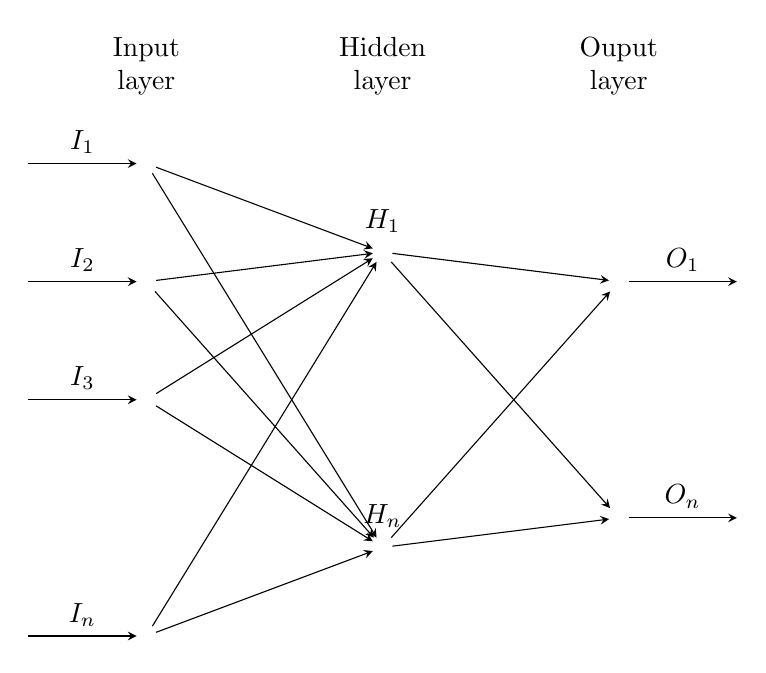
\begin{tikzpicture}[x=1.5cm, y=1.5cm, >=stealth]

    \foreach \m/\l [count=\y] in {1,2,3,missing,4}
    \node [every neuron/.try, neuron \m/.try] (input-\m) at (0,2.5-\y) {};

    \foreach \m [count=\y] in {1,missing,2}
    \node [every neuron/.try, neuron \m/.try ] (hidden-\m) at (2,2-\y*1.25) {};

    \foreach \m [count=\y] in {1,missing,2}
    \node [every neuron/.try, neuron \m/.try ] (output-\m) at (4,1.5-\y) {};

    \foreach \l [count=\i] in {1,2,3,n}
    \draw [<-] (input-\i) -- ++(-1,0)
    node [above, midway] {$I_\l$};

    \foreach \l [count=\i] in {1,n}
    \node [above] at (hidden-\i.north) {$H_\l$};

    \foreach \l [count=\i] in {1,n}
    \draw [->] (output-\i) -- ++(1,0)
    node [above, midway] {$O_\l$};

    \foreach \i in {1,...,4}
    \foreach \j in {1,...,2}
    \draw [->] (input-\i) -- (hidden-\j);

    \foreach \i in {1,...,2}
    \foreach \j in {1,...,2}
    \draw [->] (hidden-\i) -- (output-\j);

    \foreach \l [count=\x from 0] in {Input, Hidden, Ouput}
    \node [align=center, above] at (\x*2,2) {\l \\ layer};

    \end{tikzpicture}
\end{frame}

\begin{frame}
    \frametitle{Approach}
    % Your approach to solving the problem
    \framesubtitle{How will I tackle this?}
    % Why do you want to solve this problem? Previous work, and how it relates to what you are doing
    %More content goes here
\end{frame}

\begin{frame}
    \frametitle{Current Progress}
    % Your approach to solving the problem
    % How will I Judge the outcome of the work?
    \framesubtitle{What have I done already?}
\end{frame}

\begin{frame}
    \frametitle{Conclusion}
    \framesubtitle{A bit more information about this}
    % What did or will you accomplish?
    % What still needs to be done
    % \framesubtitle{A bit more information about this}
\end{frame}


% etc
\end{document}